%%%%%%%%%%%%%%%%%%%%%%%%%%%%%%%%%%%%%%%%%%%%%%%%%%%%%%%%%%%%%%%%%%%%%%%%%%
%
% Plantilla para libro de texto de matemáticas.
%
% Esta plantilla ha sido desarrollada desde cero, pero utiliza algunas partes
% del código de la plantilla original utilizada en apuntesDGIIM
% (https://github.com/libreim/apuntesDGIIM), basada a su vez en las plantillas
% 'Short Sectioned Assignment' de Frits Wenneker (http://www.howtotex.com),
% 'Plantilla de Trabajo' de Mario Román y 'Plantilla básica de Latex en Español'
% de Andrés Herrera Poyatos (https://github.com/andreshp). También recoge
% ideas de la plantilla 'Multi-Purpose Large Font Title Page' de
% Frits Wenneker y Vel (vel@latextemplates.com).
%
% Licencia:	
% CC BY-NC-SA 4.0 (https://creativecommons.org/licenses/by-nc-sa/4.0/)
%
%%%%%%%%%%%%%%%%%%%%%%%%%%%%%%%%%%%%%%%%%%%%%%%%%%%%%%%%%%%%%%%%%%%%%%%%%

% ---------------------------------------------------------------------------
% CONFIGURACIÓN BÁSICA DEL DOCUMENTO
% ---------------------------------------------------------------------------

%\documentclass[11pt, a4paper, twoside]{article} % Usar para imprimir
\documentclass[10pt, a4paper]{article}

\linespread{1.3}            % Espaciado entre líneas.
\setlength\parindent{0pt}   % No indentar el texto por defecto.
\setlength\parskip{7pt}

% ---------------------------------------------------------------------------
% PAQUETES BÁSICOS
% ---------------------------------------------------------------------------

% IDIOMA
\usepackage[utf8]{inputenc}
\usepackage[spanish, es-tabla, es-lcroman, es-noquoting]{babel}
\usepackage[table,xcdraw]{xcolor}
\usepackage{longtable}
\usepackage{subfigure}

% MATEMÁTICAS
\usepackage{amsmath}    % Paquete básico de matemáticas
\usepackage{amsthm}     % Teoremas
\usepackage{mathrsfs}   % Fuente para ciertas letras utilizadas en matemáticas

% FUENTES
\usepackage{newpxtext, newpxmath}   % Fuente similar a Palatino
\usepackage{FiraSans}                 % Fuente sans serif
\usepackage[T1]{fontenc}
\usepackage[italic]{mathastext}     % Utiliza la fuente del documento
                                    % en los entornos matemáticos

% MÁRGENES
\usepackage[margin=2.5cm, top=3cm]{geometry}

% LISTAS
\usepackage{enumitem}       % Mejores listas
\setlist{leftmargin=.5in}   % Especifica la indentación para las listas.

% Listas ordenadas con números romanos (i), (ii), etc.
\newenvironment{nlist}
{\begin{enumerate}
    \renewcommand\labelenumi{(\emph{\roman{enumi})}}}
  {\end{enumerate}}

%  OTROS
\usepackage[hidelinks]{hyperref}   % Enlaces
\usepackage{graphicx}   % Permite incluir gráficos en el documento
\usepackage{relsize}

% LISTINGS
\usepackage{listings}
\usepackage{xcolor}     % Permite definir y utilizar colores
\usepackage{lipsum}
\usepackage{courier}

% Fijar tabla a posición
\usepackage{array}
\newcolumntype{L}[1]{>{\raggedright\let\newline\\\arraybackslash\hspace{0pt}}m{#1}}
\newcolumntype{C}[1]{>{\centering\let\newline\\\arraybackslash\hspace{0pt}}m{#1}}
\newcolumntype{R}[1]{>{\raggedleft\let\newline\\\arraybackslash\hspace{0pt}}m{#1}}

\setcounter{MaxMatrixCols}{20}

% Colores para los bloques de código
\definecolor{codegreen}{rgb}{0,0.6,0}
\definecolor{codegray}{rgb}{0.5,0.5,0.5}
\definecolor{codepurple}{rgb}{0.58,0,0.82}
\definecolor{backcolour}{rgb}{0.95,0.95,0.92}
\lstdefinestyle{mystyle}{
	backgroundcolor=\color{backcolour!70!white},   
	commentstyle=\color{codegreen},
	keywordstyle=\color{blue},
	numberstyle=\tiny\color{codegray},
	stringstyle=\color{codepurple},
	basicstyle=\footnotesize\ttfamily,
	breakatwhitespace=false,         
	breaklines=true,                 
	captionpos=b,                    
	keepspaces=true,                 
	numbers=left,                    
	numbersep=5pt,                  
	showspaces=false,                
	showstringspaces=false,
	showtabs=false,                  
	tabsize=4
}
\lstset{style=mystyle}

\usepackage{amsmath}
\usepackage{algorithm}


\usepackage[noend]{algpseudocode}

\makeatletter
\def\BState{\State\hskip-\ALG@thistlm}
\makeatother

%\lstset{basicstyle=\footnotesize\ttfamily,breaklines=true}
%\lstset{framextopmargin=50pt,frame=bottomline}
 
% ---------------------------------------------------------------------------
% COMANDOS PERSONALIZADOS
% ---------------------------------------------------------------------------

% \equalto
\newcommand{\verteq}{\rotatebox{90}{$\,=$}}
\newcommand{\equalto}[2]{\underset{\scriptstyle\overset{\mkern4mu\verteq}{#2}}{#1}}


% ---------------------------------------------------------------------------
% COLORES
% ---------------------------------------------------------------------------

\definecolor{50}{HTML}{E0F2F1}
\definecolor{100}{HTML}{B2DFDB}
\definecolor{200}{HTML}{80CBC4}
\definecolor{300}{HTML}{4DB6AC}
\definecolor{400}{HTML}{26A69A}
\definecolor{500}{HTML}{009688}
\definecolor{600}{HTML}{00897B}
\definecolor{700}{HTML}{00796B}
\definecolor{800}{HTML}{00695C}
\definecolor{900}{HTML}{004D40}
\definecolor{ugrColor}{HTML}{c6474b}  % Usado en el título.
\definecolor{ugrColor2}{HTML}{c6474b} % Usado en las secciones.

% ---------------------------------------------------------------------------
% DISEÑO DE PÁGINA
% ---------------------------------------------------------------------------

\usepackage{pagecolor}
\usepackage{afterpage}

% ---------------------------------------------------------------------------
% CABECERA Y PIE DE PÁGINA
% ---------------------------------------------------------------------------

\usepackage{fancyhdr}   % Paquete para cabeceras y pies de página

% Indica que las páginas usarán la configuración de fancyhdr
\pagestyle{fancy}
\fancyhf{}

% Representa la sección de la cabecera
\renewcommand{\sectionmark}[1]{%
\markboth{#1}{}}

% Representa la subsección de la cabecera
\renewcommand{\subsectionmark}[1]{%
\markright{#1}{}}

% Parte derecha de la cabecera
\fancyhead[LE,RO]{\sffamily\textsl{\rightmark} \hspace{1em}  \textcolor{ugrColor2}{\rule[-0.4ex]{0.2ex}{1.2em}} \hspace{1em} \thepage}

% Parte izquierda de la cabecera
\fancyhead[RE,LO]{\sffamily{\leftmark}}

% Elimina la línea de la cabecera
\renewcommand{\headrulewidth}{0pt}

% Controla la altura de la cabecera para que no haya errores
\setlength{\headheight}{14pt}

% ---------------------------------------------------------------------------
% TÍTULOS DE PARTES Y SECCIONES
% ---------------------------------------------------------------------------

\usepackage{titlesec}

% Estilo de los títulos de las partes
\titleformat{\part}[hang]{\Huge\bfseries\sffamily}{\thepart\hspace{20pt}\textcolor{ugrColor}{|}\hspace{20pt}}{0pt}{\Huge\bfseries}
\titlespacing*{\part}{0cm}{-2em}{2em}[0pt]

% Reiniciamos el contador de secciones entre partes (opcional)
\makeatletter
\@addtoreset{section}{part}
\makeatother

% Estilo de los títulos de las secciones, subsecciones y subsubsecciones
\titleformat{\section}
  {\Large\bfseries\sffamily}{\thesection}{1em}{}

\titleformat{\subsection}
  {\Large\sffamily}{\thesubsection}{1em}{}[\vspace{.5em}]

\titleformat{\subsubsection}
  {\sffamily}{\thesubsubsection}{1em}{}

% ---------------------------------------------------------------------------
% ENTORNOS PERSONALIZADOS
% ---------------------------------------------------------------------------

\usepackage{mdframed}

%% DEFINICIONES DE LOS ESTILOS

% Nuevo estilo para definiciones
\newtheoremstyle{definition-style}  % Nombre del estilo
{}                                  % Espacio por encima
{}                                  % Espacio por debajo
{}                                  % Fuente del cuerpo
{}                                  % Identación
{\bf\sffamily}                      % Fuente para la cabecera
{.}                                 % Puntuación tras la cabecera
{.5em}                              % Espacio tras la cabecera
{\thmname{#1}\thmnumber{ #2}\thmnote{ (#3)}}  % Especificación de la cabecera

% Nuevo estilo para notas
\newtheoremstyle{remark-style}
{10pt}
{10pt}
{}
{}
{\itshape \sffamily}
{.}
{.5em}
{}

% Nuevo estilo para teoremas y proposiciones
\newtheoremstyle{theorem-style}
{}
{}
{}
{}
{\bfseries \sffamily}
{.}
{.5em}
{\thmname{#1}\thmnumber{ #2}\thmnote{ (#3)}}

% Nuevo estilo para teoremas y proposiciones
\newtheoremstyle{theorem2-style}
{}
{}
{}
{}
{\bfseries \sffamily}
{.}
{.5em}
{\thmname{#1}\thmnote{ (#3)}}

% Nuevo estilo para ejemplos
\newtheoremstyle{example-style}
{10pt}
{10pt}
{}
{}
{\bf \sffamily}
{}
{.5em}
{\thmname{#1}\thmnumber{ #2.}\thmnote{ #3.}}

% Nuevo estilo para la demostración

\makeatletter
\renewenvironment{proof}[1][\proofname] {\par\pushQED{\qed}\normalfont\topsep6\p@\@plus6\p@\relax\trivlist\item[\hskip\labelsep\itshape\sffamily#1\@addpunct{.}]\ignorespaces}{\popQED\endtrivlist\@endpefalse}
\makeatother

%% ASIGNACIÓN DE LOS ESTILOS

% Teoremas, proposiciones y corolarios
\newtheoremstyle{theorem-style}{}{}{}{}{}{}{ }{}
\theoremstyle{theorem-style}
\newtheorem*{datos}{}
\theoremstyle{theorem-style}
\newtheorem{nth}{Teorema}[section]
\newtheorem{nprop}{Proposición}[section]
\newtheorem{ncor}{Corolario}[section]
\newtheorem{lema}{Lema}[section]
\theoremstyle{theorem2-style}
\newtheorem{demostracion}{\textbf{\emph{Demostración}}}

% Definiciones
\theoremstyle{definition-style}
\newtheorem{ndef}{Definición}[section]

% Notas
\theoremstyle{remark-style}
\newtheorem*{nota}{Nota}

% Ejemplos
\theoremstyle{example-style}
\newtheorem{ejemplo}{Ejemplo}[section]

% Ejercicios y solución
\theoremstyle{definition-style}
\newtheorem{ejer}{Ejercicio}[section]

\theoremstyle{remark-style}
\newtheorem*{sol}{Solución}

\theoremstyle{remark-style}
\newtheorem*{dem}{Demostración}

%% MARCOS DE LOS ESTILOS

% Configuración general de mdframe, los estilos de los teoremas, etc
\mdfsetup{
  skipabove=1em,
  skipbelow=1em,
  innertopmargin=1em,
  innerbottommargin=1em,
  splittopskip=2\topsep,
}

% Definimos los marcos de los estilos


\mdfdefinestyle{datos-frame}{
	linewidth=2pt, %
	linecolor= ugrColor, %
	topline=false, %
	bottomline=false, %
	rightline=false,%
	leftmargin=0em, %
	innerleftmargin=1em, %
	innerrightmargin=1em,
	rightmargin=0em, %
}%
\mdfdefinestyle{nth-frame}{
	linewidth=2pt, %
	linecolor= 500, %
	topline=false, %
	bottomline=false, %
	rightline=false,%
	leftmargin=0em, %
	innerleftmargin=1em, %
  innerrightmargin=1em,
	rightmargin=0em, %
}%

\mdfdefinestyle{nprop-frame}{
	linewidth=2pt, %
	linecolor= 300, %
	topline=false, %
	bottomline=false, %
	rightline=false,%
	leftmargin=0pt, %
	innerleftmargin=1em, %
	innerrightmargin=1em,
	rightmargin=0pt, %
}%

\mdfdefinestyle{dem_mia-frame}{
	linewidth=2pt, %
	linecolor= ugrColor, %
	topline=false, %
	bottomline=false, %
	rightline=false,%
	leftmargin=0pt, %
	innerleftmargin=1em, %
	innerrightmargin=1em,
	rightmargin=0pt, %
}%

\mdfdefinestyle{ndef-frame}{
	linewidth=2pt, %
	linecolor= 500, %
	backgroundcolor= 50,
	topline=false, %
	bottomline=false, %
	rightline=false,%
	leftmargin=0pt, %
	innerleftmargin=1em, %
	innerrightmargin=1em,
	rightmargin=0pt, %
}%

\mdfdefinestyle{ejer-frame}{
	linewidth=2pt, %
	linecolor= ugrColor, %
	backgroundcolor= 50,
	topline=false, %
	bottomline=false, %
	rightline=false,%
	leftmargin=0pt, %
	innerleftmargin=1em, %
	innerrightmargin=1em,
	rightmargin=0pt, %
}%

\mdfdefinestyle{ejemplo-frame}{
	linewidth=0pt, %
	linecolor= 300, %
	leftline=false, %
	rightline=false, %
	leftmargin=0pt, %
	innerleftmargin=1.3em, %
	innerrightmargin=1em,
	rightmargin=0pt, %
	innertopmargin=0em,%
	innerbottommargin=0em, %
	splittopskip=\topskip, %
}%

% Asignamos los marcos a los estilos
\surroundwithmdframed[style=nth-frame]{nth}
\surroundwithmdframed[style=datos-frame]{datos}
\surroundwithmdframed[style=nprop-frame]{nprop}
\surroundwithmdframed[style=nprop-frame]{ncor}
\surroundwithmdframed[style=ndef-frame]{ndef}
\surroundwithmdframed[style=ejer-frame]{ejer}
\surroundwithmdframed[style=ejemplo-frame]{ejemplo}
\surroundwithmdframed[style=ejemplo-frame]{sol}
\surroundwithmdframed[style=dem_mia-frame]{demostracion}

% ---------------------------------------------------------------------------
% CONFIGURACIÓN DE LA PORTADA
% ---------------------------------------------------------------------------

\newcommand{\asignatura}{Técnicas de los Sistemas Inteligentes}
\newcommand{\universidad}{Universidad de Granada}

% ---------------------------------------------------------------------------
% FOTO DE LA PORTADA
% ---------------------------------------------------------------------------




\title{\vspace{3cm}\textcolor{ugrColor}{\textbf{{{{\Huge Práctica 1: Desarrollo de agentes basado en técnicas de búsqueda
(heurística) dentro del entorno GVGAI}}}}}}

\usepackage{tcolorbox}
\newtcolorbox{example}[2][]
{colback=ugrColor!25!white,colframe=ugrColor!90!white,
fonttitle=\bfseries, title=Enunciado~\thetcbcounter: #2,#1}

\usepackage{titling}
\include{titlepage}
\usepackage{wallpaper}
\date{10 de abril 2022}

\usepackage{graphicx}
\begin{document}

\section{Tabla con los Resultados Obtenidos}

\begin{figure}[htp]
\centering
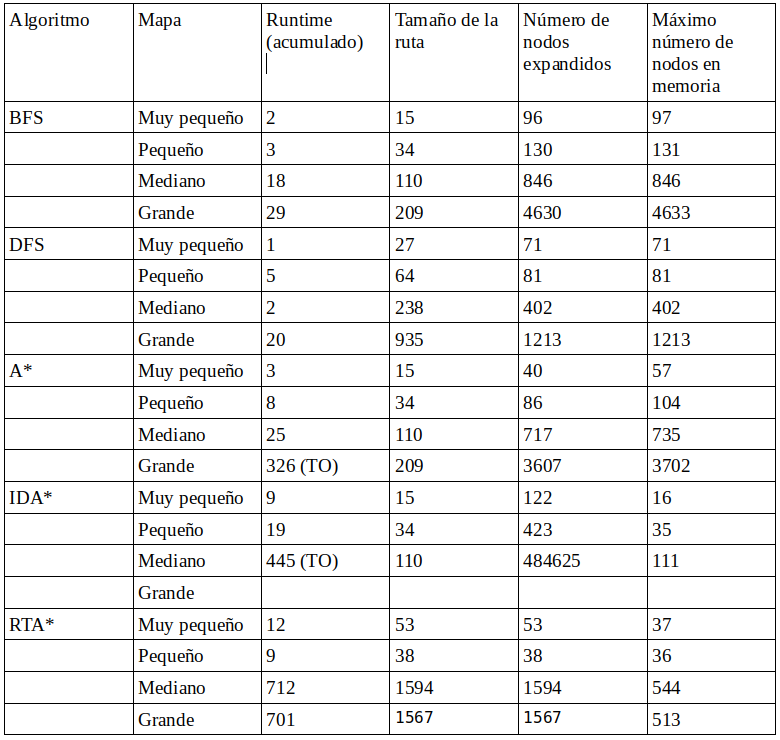
\includegraphics[scale=0.40]{tabla.png}
\caption{Tabla con los Resultados Obtenidos}
\label{}
\end{figure}

\section{Respuestas a las Preguntas Propuestas}

\subsubsection*{Entre BFS y DFS, ¿qué algoritmo puede ser considerado más eficiente de cara a
encontrar el camino óptimo?}

\textbf{Respuesta:} Analizaremos la parte teórica y práctica de cada uno de ellos a continuación. 

\textit{Runtime:} DFS es más eficiente en el caso medio que BFS. Para los valores obtenidos, podemos observar como los tiempos obtenidos suelen ser menores para DFS. Sin embargo, la diferencia no es tampoco significativamente alta. 

\textit{Tamaño de la ruta calculada:} sabemos que, teóricamente, DFS no garantiza encontrar el camino óptimo. Por su parte BFS si, puesto que el coste de desplazamiento entre nodos es constante (en nuestro caso 1). Vemos como esto se cumple en los resultados que hemos obtenido, siendo el tamaño de la ruta bastante mayor para DFS. La diferencia se hace sustancial en el último mapa principalmente. 

\textit{Número de Nodos expandidos / Consumo Memoria:} en este caso, vemos como DFS es más eficiente pues obtiene en todos los mapas un menor número de nodos expandidos y por consecuente, un menor consumo de memoria. 

Teniendo todo esto en cuenta, puesto que hablamos de encontrar el camino óptimo, me decanto por la búsqueda en anchura. Aunque DFS obtenga mejores resultados en cuanto a eficiencia, vemos como la ruta generalmente es cuanto menos óptima. Por ejemplo para el mapa grande la diferencia entre el tamaño de ruta entre DFS y BFS es de ¡¡ 726 !! Además ya hemos visto que las diferencias de tiempo no son excesivas, algo que también me hace decantarme por BFS.

\subsubsection*{¿Se podría decir que A* es más eficiente que DFS?}

\textbf{Respuesta:} Al igual que ocurría antes nos encontramos ante un algoritmo que encuentra el camino óptimo como BFS, caso de A*, y el DFS que no garantiza encontrarlo. En cuanto a lo teórico, tenemos que:

\begin{itemize}
\item \textit{Complejidad Computacional}: Para A*, esta está íntimamente relacionada con la calidad de la heurística que se utilice en el problema. En el caso peor, con una heurística de pésima calidad, la complejidad será exponencial, mientras que en el caso mejor, con una buena $h'(n)$ el algoritmo se ejecutará en tiempo lineal. Para DFS, en el peor caso, es $O(b^m)$, siendo b el factor de ramificación (número promedio de ramificaciones por nodo) y m la máxima profundidad del espacio de estados. 
\item \textit{Complejidad en Memoria: } Para DFS es $O(b^d)$, siendo b el factor de ramificación y d la profundidad de la solución menos costosa, pues cada nodo generado permanece en memoria, almacenándose la mayor cantidad de nodos en el nivel meta. En cambio, para A* dado que tiene que almacenar todos los posibles siguientes nodos de cada estado, la cantidad de memoria que requerirá será exponencial con respecto al tamaño del problema.
\end{itemize} 

Ahora pasamos a hablar de los resultados obtenidos. En cuanto a eficiencia son mejores para DFS (exceptuando el tamaño de la ruta claro). Sin embargo, esto no lo podemos tratar como el caso anterior. Esto es porque, la diferencia de tiempo para mapas sumamente grandes es significativa. Podemos ver como de hecho, A* no llega a realizar el último mapa porque excede el tiempo límite.

Es por esto que me decanto en este caso por la búsqueda en profundidad. No garantizará encontrar el camino óptimo como A*, pero nos permite encontrar un camino hasta el objetivo sin llegar a exceder el tiempo límmite. Además en cuanto al resto de características es mucho más eficiente que A*.


\subsubsection*{¿Cuáles son las principales diferencias entre A* e IDA*? ¿En qué contextos es
más conveniente usar uno u otro?}

\textbf{Respuesta:} Sabemos que ambos algoritmos encuentran, en nuestro caso, siempre los caminos óptimos. En cuanto al algoritmo A*, podemos observar como la principal ventaja que ofrece es un menor runtime que IDA*. Esto se debe en gran parte, a que el número de nodos que se expanden es significativamente menor. Para el mapa mediano, mientras que IDA* excede el timeout con un tiempo de 445, A* logra encontrar la solución con un runtime acumulado de 25ms. Diferencia notable a tener en cuenta. 

Por el contrario, uno de los puntos fuertes que presenta IDA* es que presenta un menor consumo de memoria, llegando a evidenciarse bastante a partir del mapa pequeño / mediano.

Es por esto que el uso de bien un algoritmo u otro depende de las circunstancias que se nos presenten. Es decir: 

\begin{itemize}
\item Cuando se nos exiga disponer de un algoritmo eficiente en cuanto a velocidad de cálculo, es decir, con un tiempo bajo de runtime a ser posible, nuestra elección debería ser el algoritmo de A*.
\item Por otra lado, para problemas que tengan ciertas limitaciones en cuanto al uso de memoria, pese a que tarde más, IDA* debería ser nuestra elección sin lugar a duda. 
\end{itemize}

\subsubsection*{¿Se podría decir que RTA* es más eficiente que A*?}

\textbf{Respuesta:} En esta pregunta nos encontramos ante una difícil comparación. Por un lado, A* obtiene un camino óptimo siempre pero no llega a ejecutar todos los mapas. Por el otro, nos encontramos que RTA* si consigue llegar al objetivo en todos los mapas, teniendo un menor consumo de memoria y número de nodos expandidos. La desventaja que presenta este último es la gran cantidad de tiempo que necesita. 

Entonces, teniendo en cuanto nuestros mapas de evaluación, podemos distinguir dos casos: 

\begin{itemize}
\item Para mapas similares a los 3 primeros, me decantaría por el algoritmo de A* como más eficiente. Tal y como se puede apreciar en la tabla de resultados, encuentra un camino hacia el objetivo en muchísimo menos tiempo que con RTA*. Además las diferencias en cuanto a consumo de memoria y nodos expandidos, no son muy altas. 
\item Para mapas grandes, como es el caso del último, mi elección sería RTA*. A diferencia de A* consigue ejecutar el juego sin excederse del tiempo límite. Así mismo, el consumo de memoria y los nodos expandidos son mucho menores que para A*. Luego todo son puntos a favor del algoritmo en tiempo real. 
\end{itemize}

\end{document}